\documentclass[12pt]{article}%
\usepackage{amsfonts}
\usepackage{fancyhdr}
\usepackage{comment}
\usepackage[a4paper, top=2.5cm, bottom=2.5cm, left=2.2cm, right=2.2cm]%
{geometry}
\usepackage{times}
\usepackage{amsmath}
\usepackage{changepage}
\usepackage{amssymb}
\usepackage{ifthen}
\usepackage{algorithm, algpseudocode}
\usepackage{graphicx}%
\setcounter{MaxMatrixCols}{30}
\newtheorem{theorem}{Theorem}
\newtheorem{acknowledgement}[theorem]{Acknowledgement}
%\newtheorem{algorithm}[theorem]{Algorithm}
\newtheorem{axiom}{Axiom}
\newtheorem{case}[theorem]{Case}
\newtheorem{claim}[theorem]{Claim}
\newtheorem{conclusion}[theorem]{Conclusion}
\newtheorem{condition}[theorem]{Condition}
\newtheorem{conjecture}[theorem]{Conjecture}
\newtheorem{corollary}[theorem]{Corollary}
\newtheorem{criterion}[theorem]{Criterion}
\newtheorem{definition}[theorem]{Definition}
\newtheorem{example}[theorem]{Example}
\newtheorem{exercise}[theorem]{Exercise}
\newtheorem{lemma}[theorem]{Lemma}
\newtheorem{notation}[theorem]{Notation}
\newtheorem{problem}[theorem]{Problem}
\newtheorem{proposition}[theorem]{Proposition}
\newtheorem{remark}[theorem]{Remark}
\newtheorem{solution}[theorem]{Solution}
\newtheorem{summary}[theorem]{Summary}
\newenvironment{proof}[1][Proof]{\textbf{#1.} }{\ \rule{0.5em}{0.5em}}

\newcommand{\Q}{\mathbb{Q}}
\newcommand{\R}{\mathbb{R}}
\newcommand{\C}{\mathbb{C}}
\newcommand{\Z}{\mathbb{Z}}

\begin{document}

\title{Assignment 6}
\author{Changwoon Choi \\ 2020-20206}
\date{\today}
\maketitle

\section{Model Representation}
Suppose you want to train the digit classifier using a simple neural network (i.e. the number of output nodes is 10). The input is a square gray image with 100 pixels. (i.e. (10x10) for on image). If your network has only one hidden layer with 50 nodes, how many parameters will be updated in the training phase (HINT: do not forget the bias node)?
\\

Ans) The number of  parameters between the input layer and the hidden layer is 101 x 50 = 5050, and the number of parameters between the hidden layer and the output layer is 51 x 10 = 510. $\therefore$ the number of parameters that would be updated in the training phase is 5560.

\section{Feedforward Propagation}
 You are using the neural network pictured below and have learned the parameters $\Theta^{(1)} = \begin{bmatrix}
	1 & 2.1 & 1.3 \\
	1 & 0.6 & -1.2 \\
\end{bmatrix}$ (used to compute $a^{(3)}$) and $\Theta^{(2)} = \begin{bmatrix}
	1 & 4.5 & 3.1 \\
\end{bmatrix}$  (used to compute $a^{(3)}$, as function of $a^{(2)}$). Suppose you swap the parameters for the first hidden layer between its two units. So  $\Theta^{(1)} = \begin{bmatrix}
	1 & 0.6 & -1.2 \\
	1 & 2.1 & 1.3 \\
\end{bmatrix}$and $\Theta^{(2)} = \begin{bmatrix}
	1 & 4.5 & 3.1 \\
\end{bmatrix}$. How will this change the value of the output $h_{\Theta}(x)$ ? 
\begin{figure}[h]
	\centering
	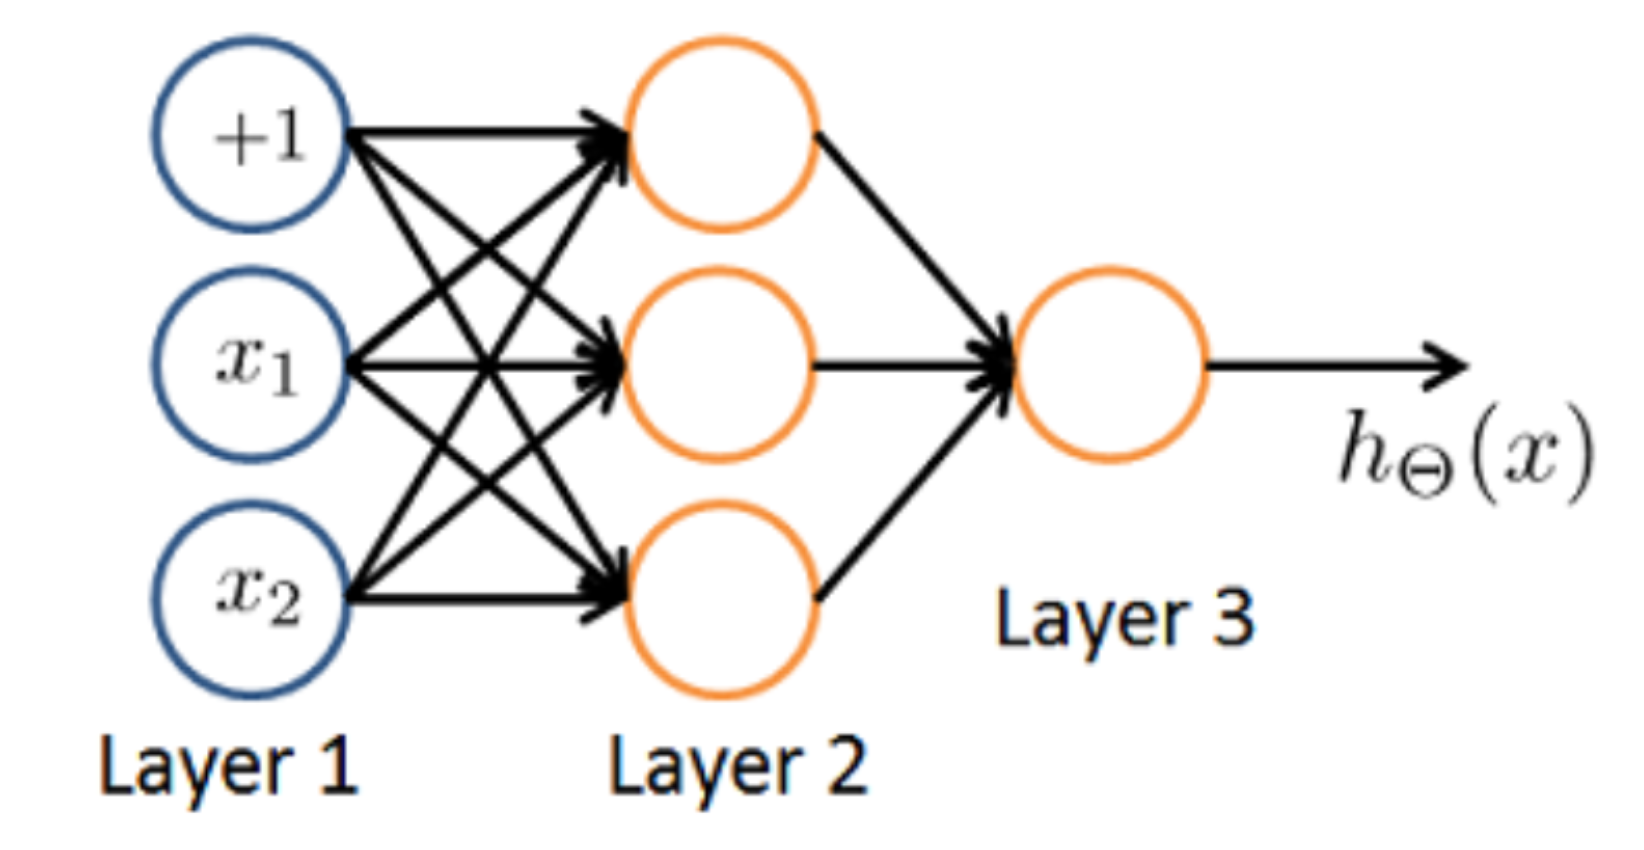
\includegraphics[scale=0.3]{HW6_fig1.png}
\end{figure}
\\
Ans) d. Insufficient information to tell: it may increase or decrease. It is depend on $x$. (If the parameters were trained well, it may be increase, but it is not guaranteed.)

\section{Back Propagation}
When training the neural networks, what are the typical steps for using a gradient descent algorithm?\\
1) Compute the error between the actual value and the predicted value\\
2) Reiterate until you find the best weights of network (until the error is sufficiently small)\\
3) Pass an input through the network and get values from output layer\\
4) Initialize random weight and bias\\
5) Go to each neuron which contributes to the error and change its respective values to reduce the error\\

Ans) c. 4 $\rightarrow$ 3 $\rightarrow$ 1 $\rightarrow$ 5 $\rightarrow$ 2

\section{Gradient Computation}
Given a quadratic cost function $J(\Theta) = {1 \over 2} \sum_{k \in K} ((h_\Theta (x)_k - y_k ))^2$ and  ``error" of cost for $a^{(l)}_j$ (unit $j$ in layer $l$) $\delta^{(l)}_j = {\partial \over {\partial z^{(l)}_j}} J(\Theta)$, drive the following equations:
\subsection{$\delta^{(L)} = (a^{(L)} - y).*g^{'}(z^{(L)})$}
Ans) let $e^{(L)}_j = g(z^{(L)}_j) - y_j$. and by a simple chain rule, 
\begin{equation}
	\begin{aligned}
		\delta^{(L)}_j & = {\partial \over {\partial z^{(L)}_j }} J(\Theta) \\
		& = {\partial J(\Theta) \over {\partial e^{(L)}_j }} {\partial e^{(L)}_j \over {\partial g(z^{(L)}_j ) }} {\partial g(z^{(L)}_j ) \over {\partial z^{(L)}_j }} \\
		& = {\partial \over {\partial e^{(L)}_j }} ({1 \over 2} \sum_{k \in K} {e^{(L)}_k}^2 ) {\partial \over {\partial g(z^{(L)}_j )}} ( g(z^{(L)}_j) - y_j) {\partial \over {\partial z^{(L)}_j}} (g(z^{(L)}_j))\\
		& =  e^{(L)}_j g^{'}(z^{(L)})
	\end{aligned}
\end{equation}
$\therefore \delta^{(L)} = (a^{(L)} - y)g^{'}(z^{(L)})$

\subsection{$\delta^{(l)} = (\Theta^{(l)})^{T} \delta^{(l+1)}.*g^{'}(z^{(l)})$}
Ans) let $e^{(l)}_j = g(z^{(l)}_j) - y_j$. and by a simple chain rule, 
\begin{equation}
	\begin{aligned}
		\delta^{(l)}_j & = 
	\end{aligned}
\end{equation}
\subsection{$\frac{\partial}{\partial \Theta_{ij}^{(l)}} J(\Theta) = a_{j}^{(l)} \delta_{i}^{l+1}$}

\section{Gradient Computation}
Repeat Problem 4 for the cross-entropy cost function
\subsection{$\delta^{(L)} = (a^{(L)} - y).*g^{'}(z^{(L)})$}
\subsection{$\delta^{(l)} = (\Theta^{(l)})^{T} \delta^{(l+1)}.*g^{'}(z^{(l)})$}
\subsection{$\frac{\partial}{\partial \Theta_{ij}^{(l)}} J(\Theta) = a_{j}^{(l)} \delta_{i}^{l+1}$}

\section{Convexity of Cost Functions}
Assume we use a sigmoid function for output layer activation in Neural Network; i.e. $a_L = g_L (z_L ) = {1 \over {1 + e^{(-zL)}}}$, Prove that the cross-entropy loss function is convex.\\
Ans) Recall the cross-entropy loss:
\begin{equation}
	J(\mathbf{w}) = - (\sum_{i=1}^{m} y_i \log(g(\mathbf{w^T x_i})) + (1 - y_i )\log (1 - g(\mathbf{w^T x_i})))
\end{equation}
where $g(z) = 1/(1+e^{-z})$ and $g'(z) = g(z) (1 - g(z))$.\\
let's show that $- \log(g(\mathbf{w^T x}))$ and $- \log(1 - \mathbf{w^T x}))$ are convex in $\mathbf{w}$:\\
\begin{equation}
	\begin{aligned}
		\nabla_\mathbf{w} (- \log g(\mathbf{w^T x})) &= - {{\nabla_\mathbf{w} (g(\mathbf{w^T x}))} \over {g(\mathbf{w^T x})}}\\
		&= - { {g'(\mathbf{w^T x}) \nabla_\mathbf{w} (\mathbf{w^T x})} \over {g(\mathbf{w^T x})}} \\
		&= (g(\mathbf{w^T x}) - 1) \mathbf{x}\\
	\end{aligned}
\end{equation}
\begin{equation}
	\begin{aligned}
		\nabla^2_\mathbf{w} (- \log g(\mathbf{w^T x}))&= \nabla_w (g(\mathbf{w^T x}) \mathbf{x})\\
		&=g(\mathbf{w^T x})(1 - g(\mathbf{w^T x}))\mathbf{x x^T}
	\end{aligned}
\end{equation}
$\because$ $g$ is sigmoid function, $g(\mathbf{w^T x})$ is between 0 and 1.\\
$\therefore$ the matrix is positive semi-definite for any $\mathbf{x}$.\\
Similarly we can show that
\begin{equation}
	\nabla_\mathbf{w} (- \log (1 - g(\mathbf{w^T x}))) = g(\mathbf{w^T x})\mathbf{x} 
\end{equation}
\begin{equation}
	\nabla_w^2(- \log (1 - g(\mathbf{w^T x}))) = g(\mathbf{w^T x})(1 - g(\mathbf{w^T x}))\mathbf{x x^T}
\end{equation}
and, it is positive semi-definite for any $\mathbf{x}$.\\
$\therefore$ $J(\mathbf{w})$ is convex in $\mathbf{w}$.
\end{document}
